\section{Using the DR25 Catalog for Occurrence Rate Calculations}
\label{s:occurates}
The DR25 candidate catalog was designed with the goal of providing a well characterized sample of planetary candidates for use in occurrence rate calculations.  For those smallest planets at the longest periods, our vetting is especially prone to miss transits and confuse other signals as transits, and this must be accounted for when doing occurrence rates.  However, the completeness and reliability presented in this paper are simply the last two pieces of a much larger puzzle that must be assembled in order to perform occurrence rates with this catalog.  In this section we endeavor to make users aware of other issues and biases, as well as all the products available to help interpret this KOI catalog, all of which are hosted at the NASA exoplanet archive. 

%\subsection{Pipeline Detection Efficiency}
%Any measure of the catalog completeness must include the completeness of the Robovetter and the \Kepler{} Pipeline.  The Pipeline's detection efficiency has been explored in two ways: using pixel-level transit injection and using flux-level transit injection.  Pixel level transit injection gives an average response of the transit-search over all the stars that were searched. A full description of the signals that were injected and recovered can be found in \citet{Christiansen2017}.  To understand the recoverability of transiting planets on individual targets, 600,000 (or 2,000) transiting signals were injected on individual stars to see which ones would be recovered by TPS.  This led to an understanding of how to identify those stars that deviate from the average detection efficiency measured from the pixel-level injection.  The pixel-level measurements have the advantage of following transit signals through all processing steps of the \Kepler{} Pipeline, and the recovered signals can be further classified with the Robovetter, as demonstrated in \S\ref{s:candr}.  However, since the pixel-level injection only includes one injection per target, it does not elucidate individual-target variations in pipeline completeness due to differences in stellar properties or astrophysical variability. The flux-level injections revealed  that  there  are  significant target-to-target variations in the detection efficiency. The flux-level injections and the resulting detection efficiency is available for the sample of stars that were part of this study. For more information on the flux-level injection study see \citet{Burke2017c}. All products associated with the flux-level and pixel-level injections can be found at NExScI.\footnote{\url{https://exoplanetarchive.ipac.caltech.edu/docs/KeplerSimulated.html}}

\subsection{Pipeline Detection Efficiency}

Any measure of the catalog completeness must include the completeness of the Robovetter and the \Kepler{} Pipeline. The Pipeline's detection efficiency has been explored in two ways: using pixel-level transit injection and using flux-level transit injection. In the former, a simulated transiting planet signal is injected into the calibrated pixels of each Kepler target, which are then processed through the pipeline. This experiment provides an estimate of the average detection efficiency over all the stars that were searched. A full description of the signals that were injected and recovered can be found in \citet{Christiansen2017}. The pixel-level measurements have the advantage of following transit signals through all the processing steps of the \Kepler{} Pipeline, and the recovered signals can be further classified with the Robovetter, as demonstrated in \S\ref{s:candr}. Figure \ref{f:fulldetectionefficiency} shows the average pipeline detection efficiency for a sample of FGK stars: the left panel shows the pipeline detection efficiency, and the right panel shows the combined Pipeline and Robovetter detection efficiency, calculated by taking the injections that were successfully recovered by the pipeline and processing them through the Robovetter. 
{\color{blue}A gamma cumulative distribution function is fit to both \citep[see equation 1 of ][]{Christiansen2016}.  Notice that the detection efficiency decreases by 5--10~percentage points (of the entire set that were injected) for all MES, as expected given the results shown in Figure~\ref{f:1dcompare}. }



Since the pixel-level transit injection includes only one injection per target, it does not examine potential variations in the pipeline completeness for individual targets due to differences in stellar properties or astrophysical variability. To probe these variations, a small number of individual stars had a large number of transiting signals (either several thousand or several hundred thousand, depending on the analysis) injected into the detrended photometry, which was processed only through the transit-search portion of the TPS module. The flux-level injections revealed that there are significant target-to-target variations in the detection efficiency. The flux-level injections and the resulting detection efficiency is available for the sample of stars that were part of this study. For more information on the flux-level injection study see \citet{Burke2017c}. All products associated with the flux-level and pixel-level injections can be found at NExScI.\footnote{\url{https://exoplanetarchive.ipac.caltech.edu/docs/KeplerSimulated.html}}


\begin{figure*}[ht]
\centering
\hspace{-2.5em}\begin{tabular}{cc}
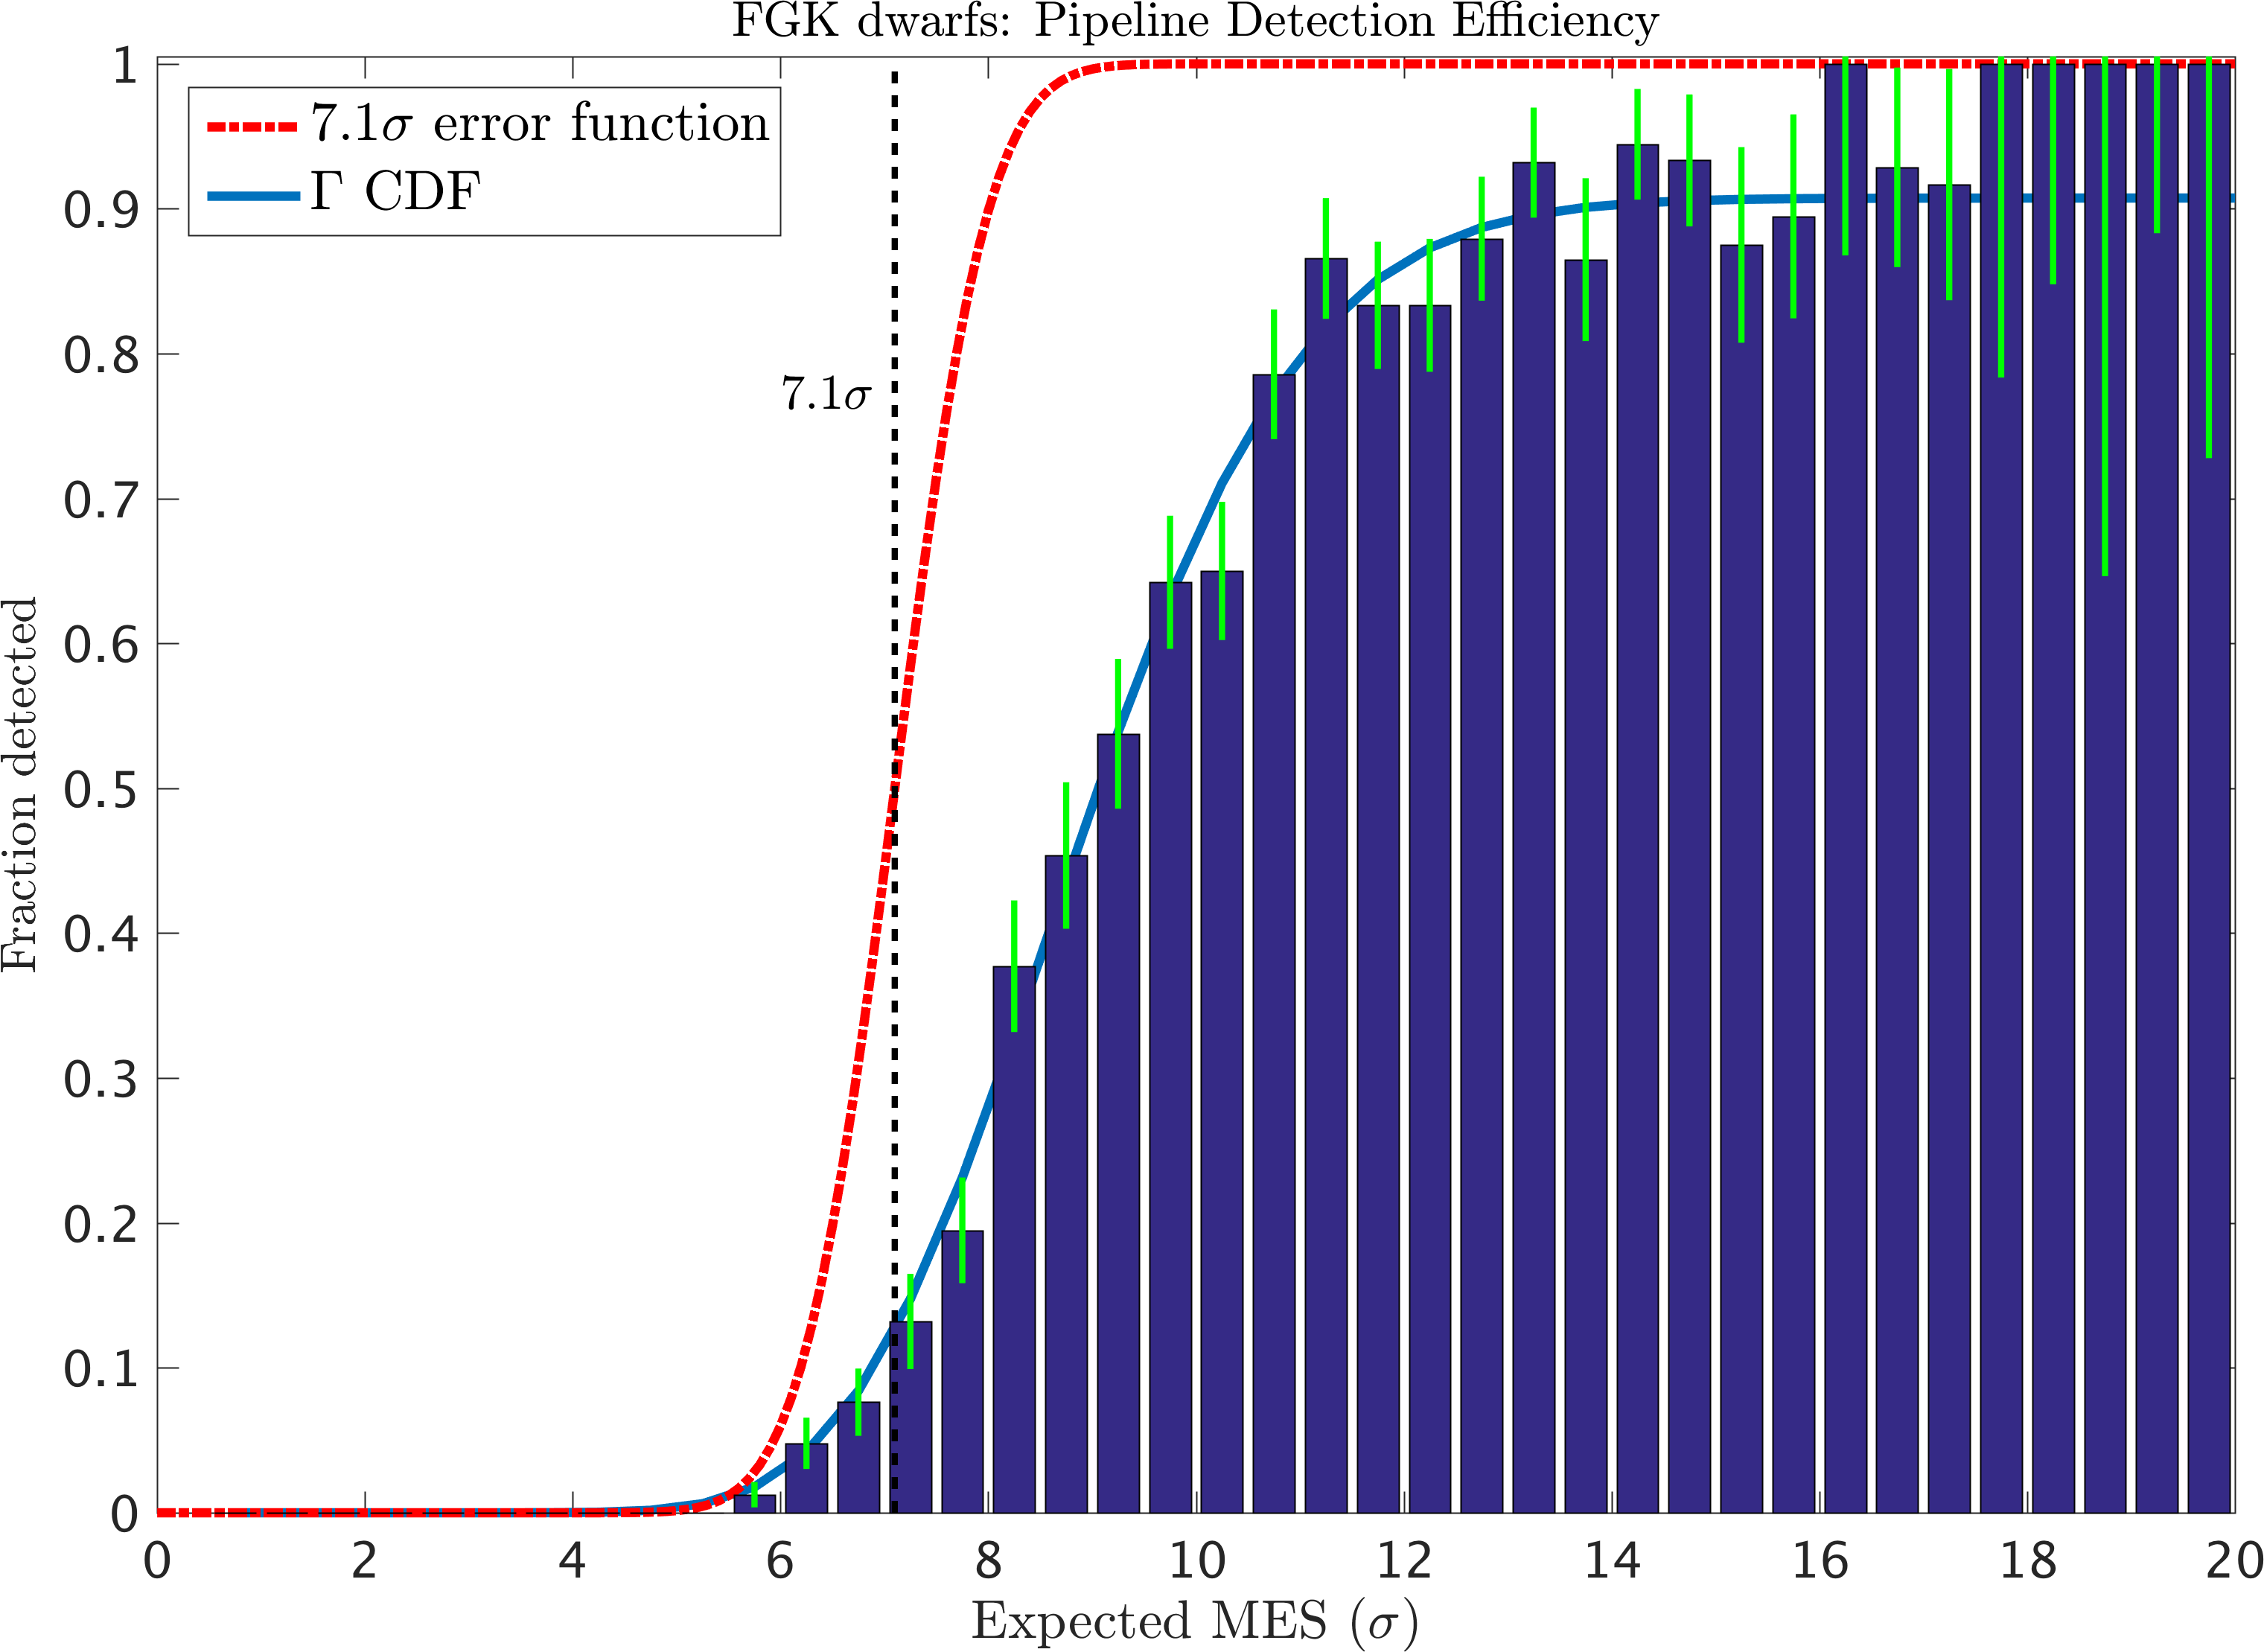
\includegraphics[width=0.5\linewidth]{fig-senscurvwithfits_withoutRv-trimmed.png} &
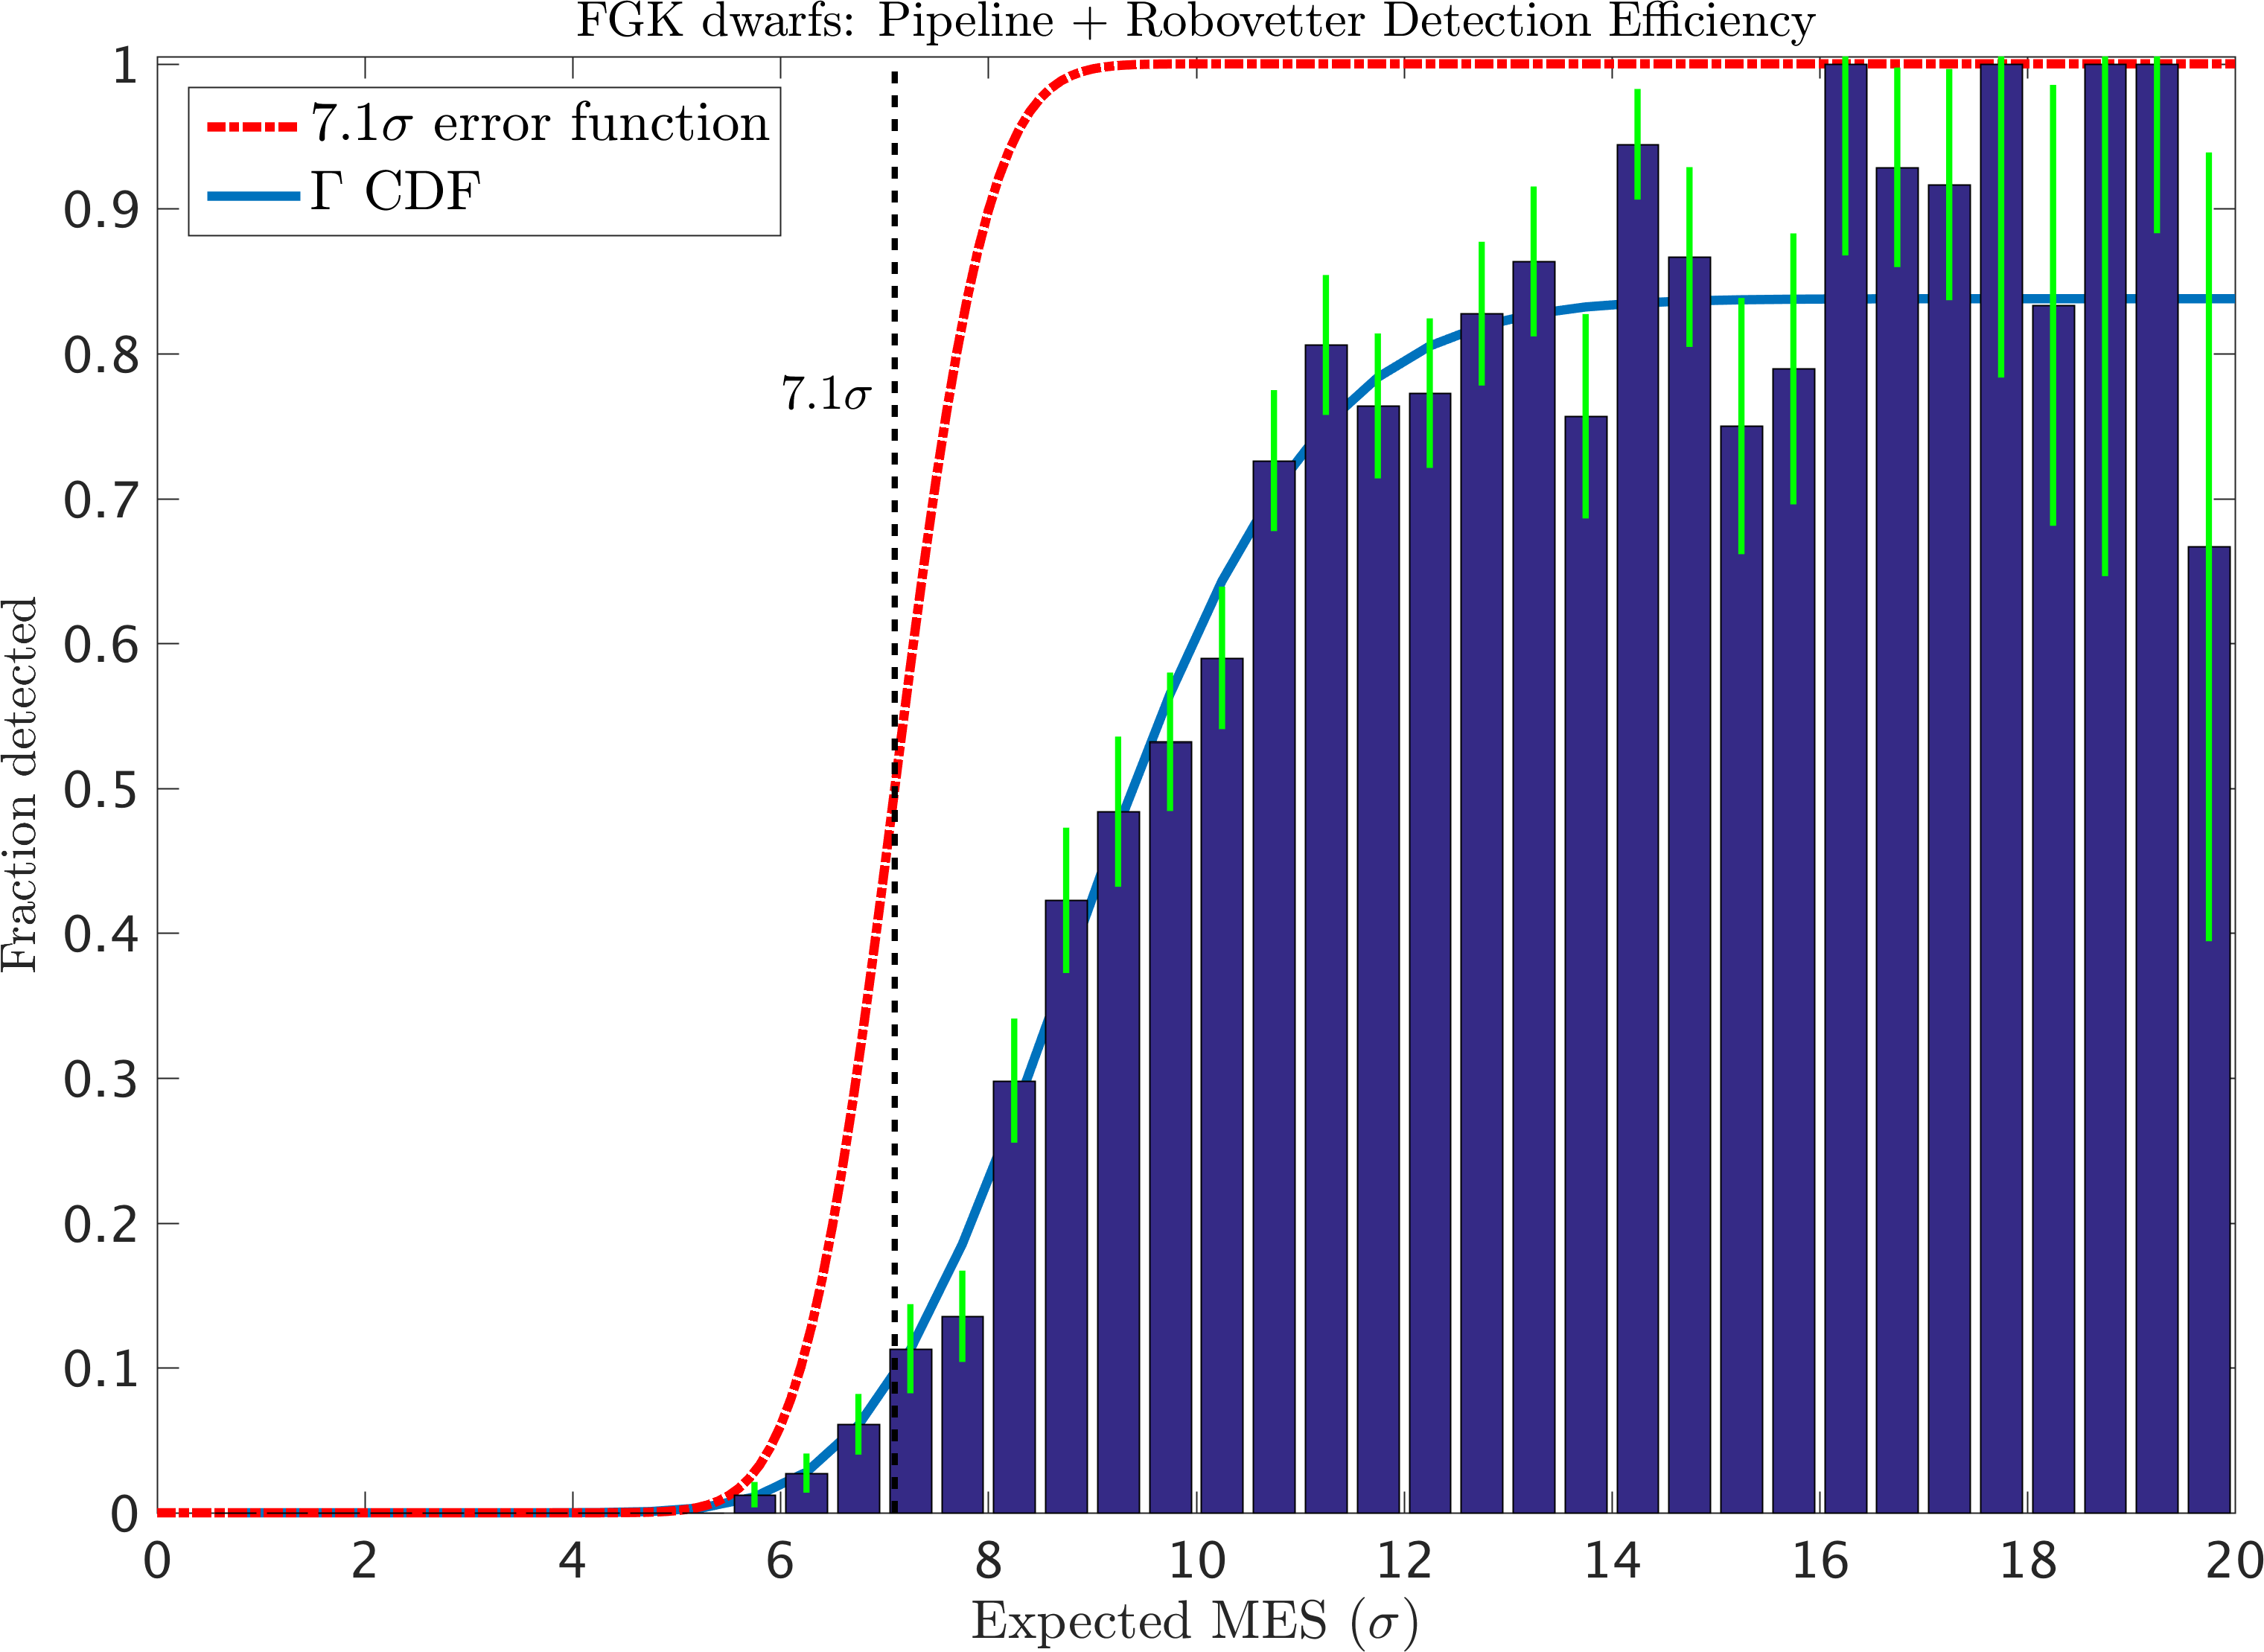
\includegraphics[width=0.5\linewidth]{fig-senscurvwithfits_withRv-trimmed.png}
\end{tabular}
\caption{Left: The average detection efficiency of the pipeline for a sample of FGK stars, as measured by the pixel-level transit injection experiment and described by \citet{Christiansen2017}. The solid blue line is a best-fit $\Gamma$ cumulative distribution function \citep[see Equation 1 of ][]{Christiansen2016}; the red dashed line shows the hypothetical performance for a perfect detector in TPS. Right: The average detection efficiency of the \Kepler{} Pipeline and the Robovetter, where the injections successfully recovered by the Pipeline are then subsequently evaluated as PCs by the Robovetter.}

\label{f:fulldetectionefficiency}

\end{figure*}


\subsection{Astrophysical Reliability}
We have described the reliability of the DR25 candidates with regard to the possibility that the observed events are actually caused by stellar or instrumental noise. See \S\ref{s:candr} for how this reliability varies with various measured parameters.  Even if the observed signal is real, other astrophysical events can mimic a transit \citep[see e.g.][]{Morton2016}. Some of these other astrophysical events are removed by carefully vetting the KOI with \Kepler{} data alone.  Specifically, the Robovetter looks for significant secondary eclipses to rule out eclipsing binaries, and for a significant offset in the location of the in- and out-of-transit centroids to rule out background eclipsing binaries. Using the pixel-level transit injection, we inject signals that mimic eclipsing binaries and signals that mimic background eclipsing binaries. Those that were recovered by the \Kepler{} Pipeline can be used to measure the effectiveness of the Robovetter at removing this type of false positive. A full description of these injections and an analysis of the Robovetter's effectiveness in detecting these signals can be found in \citet{Coughlin2017a}.

To further evaluate the effectiveness of the centroid Robovetter and to more robustly determine whether a KOI's signal originates from the target star, see the Astrophysical Positional Probabilities Table\footnote{\url{https://exoplanetarchive.ipac.caltech.edu/cgi-bin/TblView/nph-tblView?app=ExoTbls&config=koiapp}}.  Using a more complete catalog of stars than the original Kepler Input Catalog \citet{Brown2011}, \citet{Bryson2017a} calculates the probability that the observed transit-like signal originates from the target star. Note, these positional probabilities are computed independently of the results from the Centroid Robovetter, and are not used by the Robovetter. 

Additional information on Robovetter effectiveness can be gathered by using the Certified False Positive table at the NASA Exoplanet Archive\footnote{\url{https://exoplanetarchive.ipac.caltech.edu/cgi-bin/TblView/nph-tblView?app=ExoTbls\&config=fpwg}} which uses follow-up observations and information from sources outside \kepler{}, combined with detailed human vetting, to determine which KOIs are truly false positives. The Robovetter effectiveness can be combined with the \emph{a priori} occurrence rates of the different types of astrophysical events to determine the astrophysical reliability of planet candidates. The results of the vespa code \citep[][]{Morton2016}, which compares the likelihood that a signal comes from a transit to that of one of these other astrophysical scenarios, are available in the Astrophysical False Positive Probabilities Table\footnote{\url{https://exoplanetarchive.ipac.caltech.edu/cgi-bin/TblView/nph-tblView?app=ExoTbls\&config=koifpp}} for the KOIs. 



\subsection{Imperfect Stellar Information}
For those doing occurrence rates, another issue to consider is whether the measured size of the planet is correct. The stellar catalog (i.e., radii and temperatures) provided by \citet{Mathur2017ApJS} collates the best information about the \Kepler{} stars available at the time, but typically has errors of 27 percent for the stellar radii. Results from \textit{Gaia} \citep{gaia2,gaia1} are expected to fix many of shortcomings of this catalog. Another issue, studied by \citet{Ciardi2015} and again by \citet{Furlan2017}, finds that $\sim$30\% of KOI host stars are part of a bound or line-of-sight binary within one \Kepler{} pixel (3.98$\arcsec$) of the primary star. While the \Kepler{} Pipeline does account for stray light in the aperture from stars listed in the \Kepler{} Input Catalog \citep{Brown2011}, many of these binaries are only known because of recent high resolution imaging. As a result the observed transits are diluted by unaccounted for stars. In these cases the planet size is actually larger than measured because the added flux suppresses the depth measurement. For occurrence rates this also affects the stars that have no planets because it means the search did not extend to planet radii that are as small as the stellar catalog indicates.  For this reason, any correction based on light from observed binaries needs to be applied across all searched stars, not just the planet hosts.


%The reliability of individual objects against can be better understood by consulting the 

%Do I need to mention APP and FPWG. I don't quite see how to use them for getting a handle on reliability. 
%Several tools are also available to understand whether an individual target is likely caused by an astrophysical source. the reliability of the The probabilities provided in the APP table measure how likely it is that a star’s location matches the location of the transit signal – they do not measure the probability that the transit signal is consistent with a planet orbiting that star.